\documentclass[11pt,a4paper]{article}

\usepackage[utf8]{inputenc}
\usepackage[MeX]{polski}
\usepackage{graphicx}
\usepackage{wrapfig}
\usepackage{color}
\usepackage{amsmath}
\usepackage{amssymb}
\usepackage[inkscapelatex=false]{svg}
\usepackage{array, makecell}
\usepackage{mhchem}
\usepackage{tabularx}
\usepackage{braket}
\usepackage{pdfpages}

\usepackage{multicol}
\usepackage{colortbl}
\usepackage[Export]{adjustbox}
\adjustboxset{max size={0.9\linewidth}{0.9\paperheight}}
\usepackage[colorlinks=true,linkcolor=red,citecolor=green]{hyperref}

\textwidth=16cm
\textheight=23cm
\topmargin=-2cm
\oddsidemargin=0cm

\setlength{\parskip}{0.6em}
\setlength{\jot}{12pt}

\renewcommand{\arraystretch}{1.4}
\renewcommand\theadfont{\bfseries}

\newcommand{\todo}[1]{\textcolor{red}{TODO: #1}}

\begin{document}

\title{Ising model on random graphs with non-limited range of interactions}
\author{Dawid Karpiński,\\Supervisor: dr inż. Krzysztof Suchecki}
\date{}
\maketitle

\section*{Abstract}

The Ising model, renowned for its simplicity and effectiveness in capturing phase transitions, serves as a powerful tool to analyze the emergent properties of complex systems. The core objective of this research is to unravel the implications of non-limited interaction ranges in the context of random graphs. Traditional Ising models often assume a fixed range of interactions among neighboring spins. This work challenges that assumption by considering scenarios where interactions extend beyond the nearest neighbors, incorporating a broader and more realistic perspective on the interplay between spins.

\section{Introduction}

Historically, the Ising model has played a crucial role in the development of statistical mechanics and the understanding of critical phenomena. The starting point - one-dimensional Ising model - was solved exactly by Ernst Ising's advisor, Wilhelm Lenz, in 1920. However, the two-dimensional case remained unsolved for many years until the solution has been found independently by Lars Onsager in 1944, marking a significant breakthrough.


\subsection{The Ising model}

It serves as a basic model for understanding phase transitions in physical systems. In its simplest form, the model considers a lattice of discrete spins, that represent magnetic moments. These spins can be either "up" (+1) or "down" (-1), corresponding to the two possible magnetic states $s_{ij}\in\{-1, +1\}$.

The energy of the system is determined by the interactions between neighboring spins. The model assumes that each spin interacts with its nearest neighbors, and the total energy of the system depends on the alignment of these spins relative to each other.

The Hamiltonian $H$ of such model can therefore be described as:

\begin{equation}
    H = -\frac12\sum_{\langle i,j \rangle} J_{ij} s_i s_j + \mu\sum_i h_i s_i
\end{equation}

Depending on the sign of an interaction constant $J$, the evolution of the system differs. Hence, in case of $J>0$ (ferromagnetic interaction), if neighboring spins are aligned in the same direction, the energy is lowered, and if they are aligned oppositely, the energy is increased. However, when $J<0$, indicating  an antiferromagnetic interaction, the dynamics of the model undergo a reversal.


\subsection{Random graphs}

Since then, the model has been successively extended and applied to various disciplines beyond physics. There exist various ways of extending the model.

One could for instance change the topography of the spin lattice. By employing the Ising model on random graphs, one can study e.g. how information spreads through a social network, shedding light on the mechanisms that govern the diffusion of ideas, opinions, or trends within these complex systems. This approach not only contributes to the understanding of social dynamics but also showcases the versatility of the Ising model in capturing the essence of diverse real-world scenarios.

\todo{exemplary graph figure}

For this thesis, I have chosen to focus my analysis on an Erdős-Renyi graph $G_{N,p}$. Such network is constructed by choosing a number of edges for each node, with some probability described by a parameter $p$. Moreover, the average number of nearest neighbors for each node is given by the following equation:

\begin{equation}
    \braket{k} = (N-1) \cdot p
\end{equation}

\section{Motivation}

\section{Literature Review}
\begin{itemize}
\item review existing literature on the Ising model
\end{itemize}

\section{Analytical mean-field approximation for critical temperature}

\section{Simulation}

\subsection{Methodology}

\subsection{Results and Discussion}

\todo{differences between J generation methods with k constant}

\section{Conculsion}

% \begin{figure}[ht!]
%     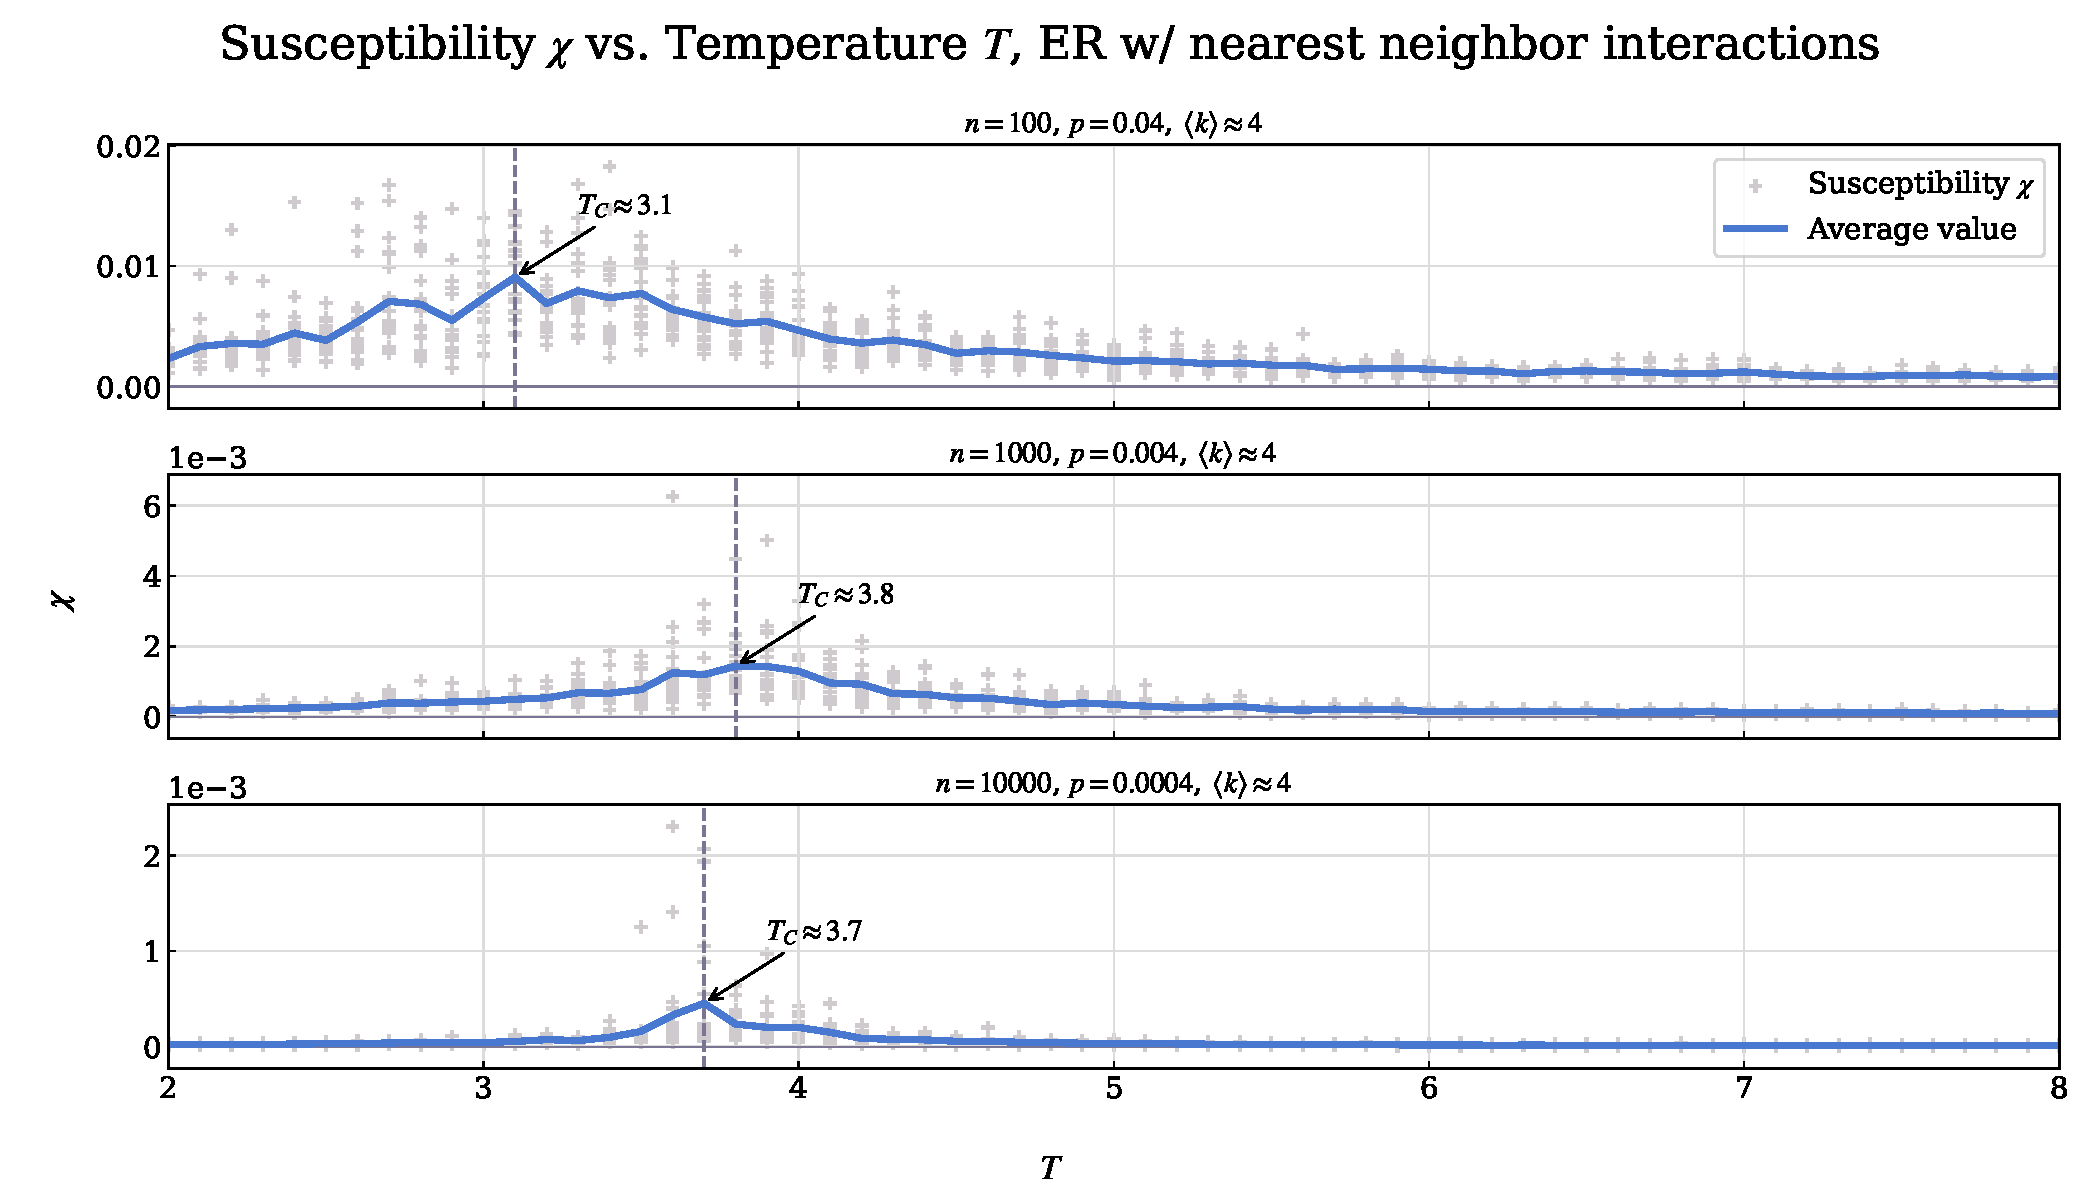
\includegraphics[width=\textwidth]{../figures/suscept_ER_nearest.pdf}
% \end{figure}
%
% \begin{figure}[ht!]
%     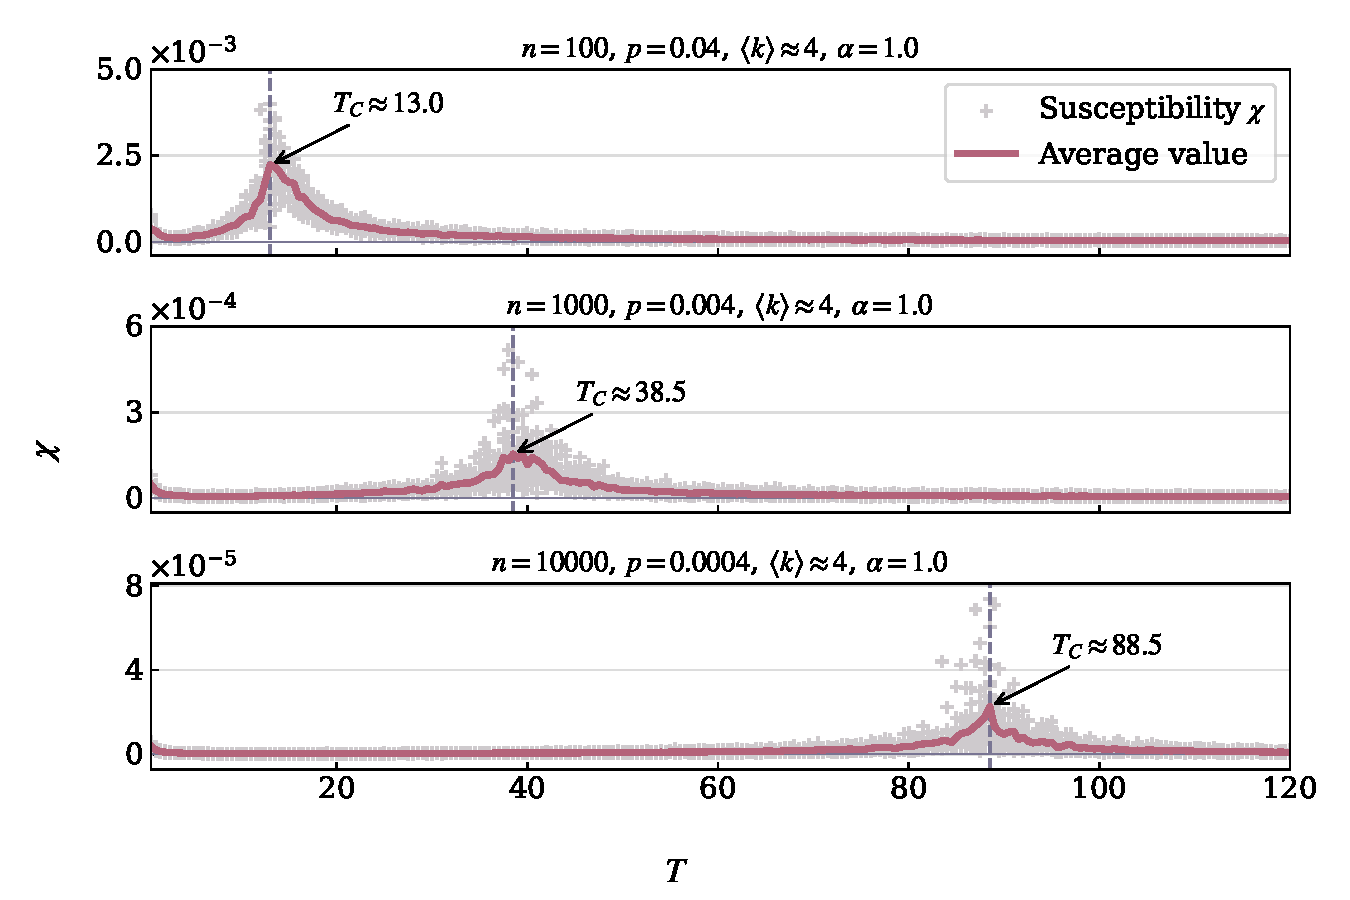
\includegraphics[width=\textwidth]{../figures/suscept_ER_single.pdf}
% \end{figure}
%
% \begin{figure}[ht!]
%     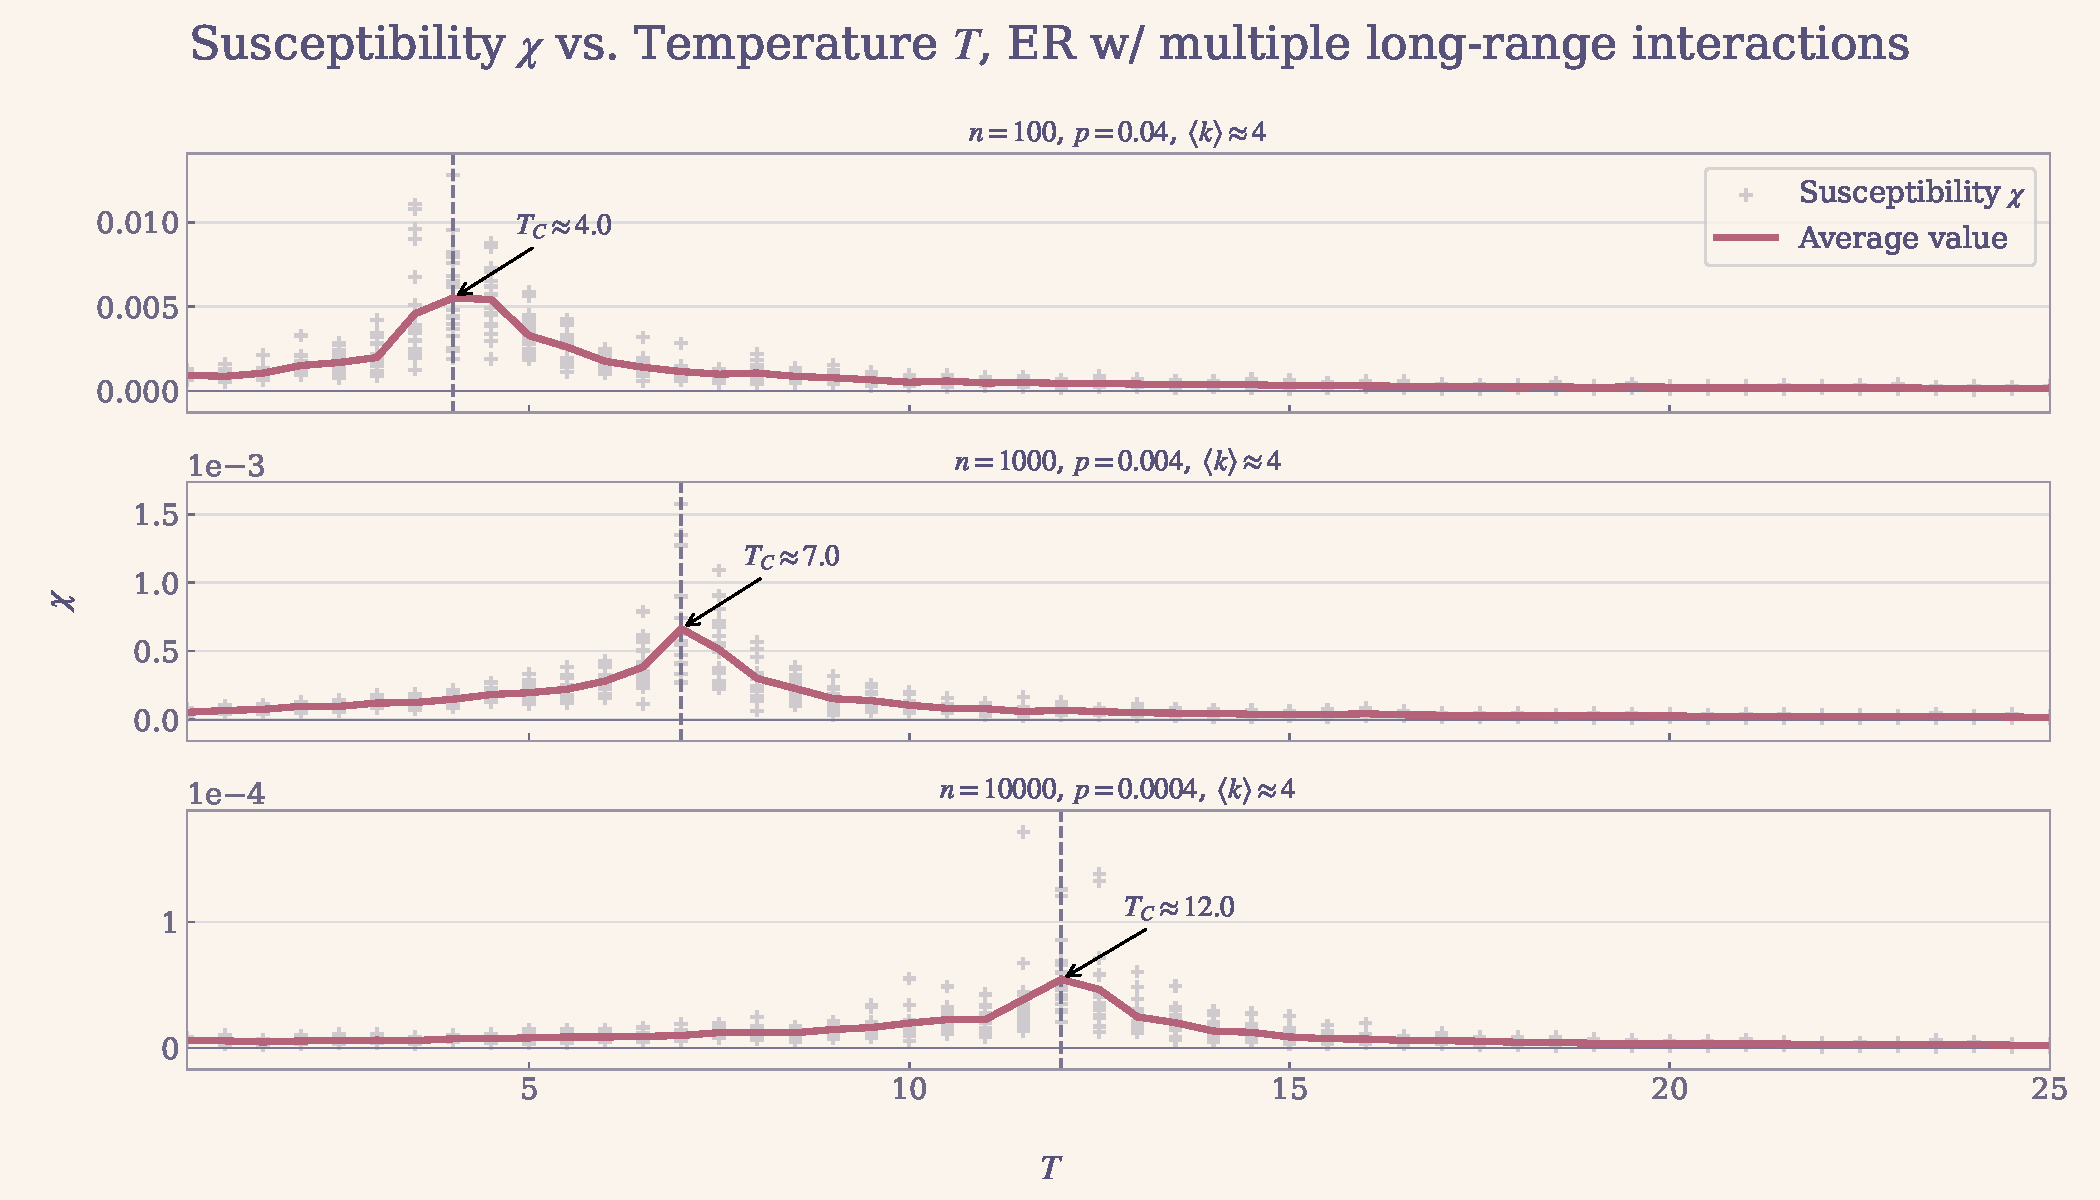
\includegraphics[width=\textwidth]{../figures/suscept_ER_multiple.pdf}
% \end{figure}

\todo{$T_C$ vs. k with n kept constant}
\begin{figure}[ht!]
    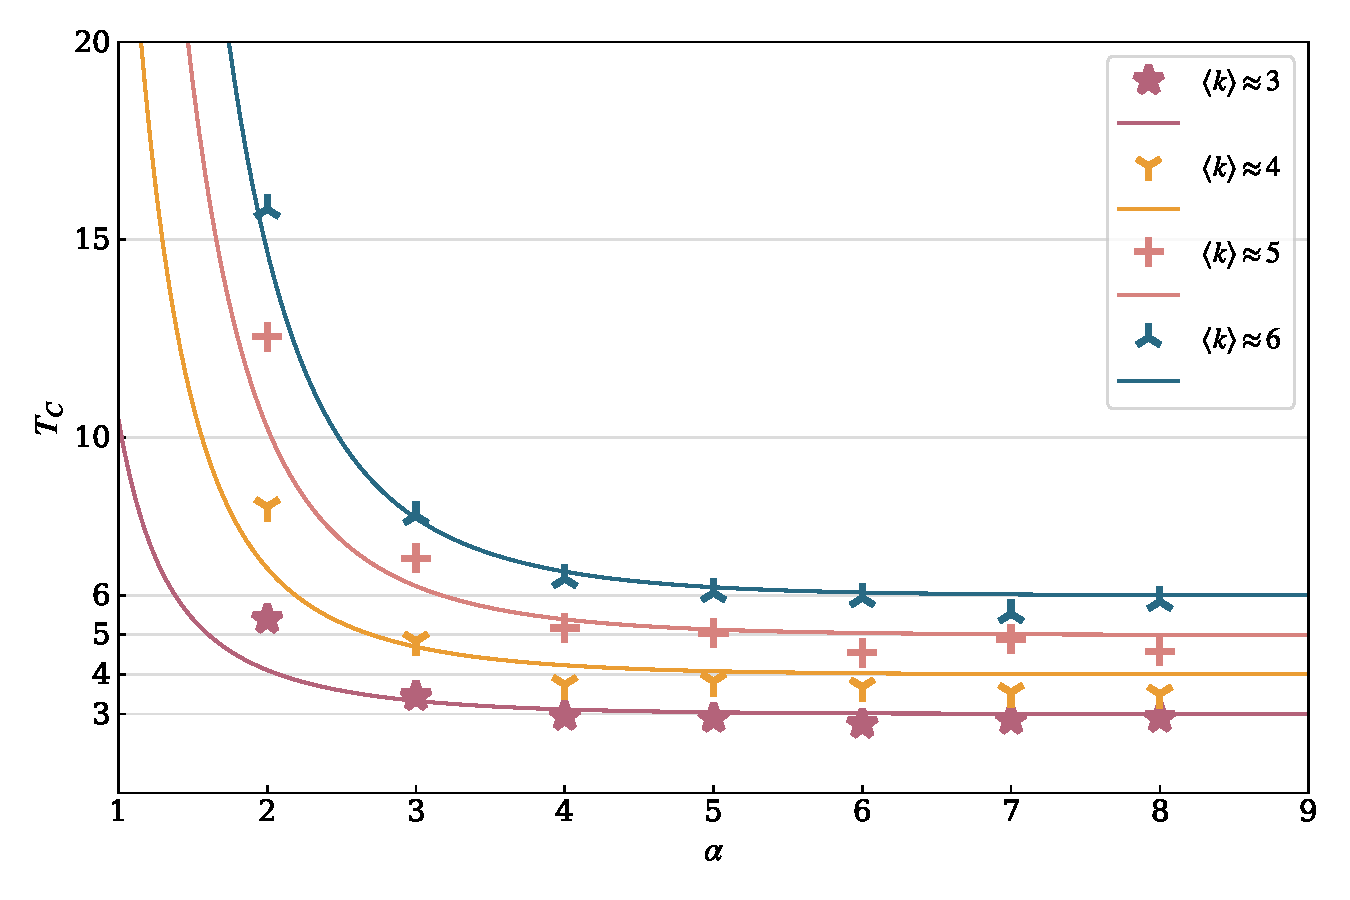
\includegraphics[width=\linewidth]{../figures/TC_vs_alpha.pdf}
\end{figure}

\todo{$T_C$ vs. $\alpha$ for exponential decay}
\begin{figure}[ht!]
    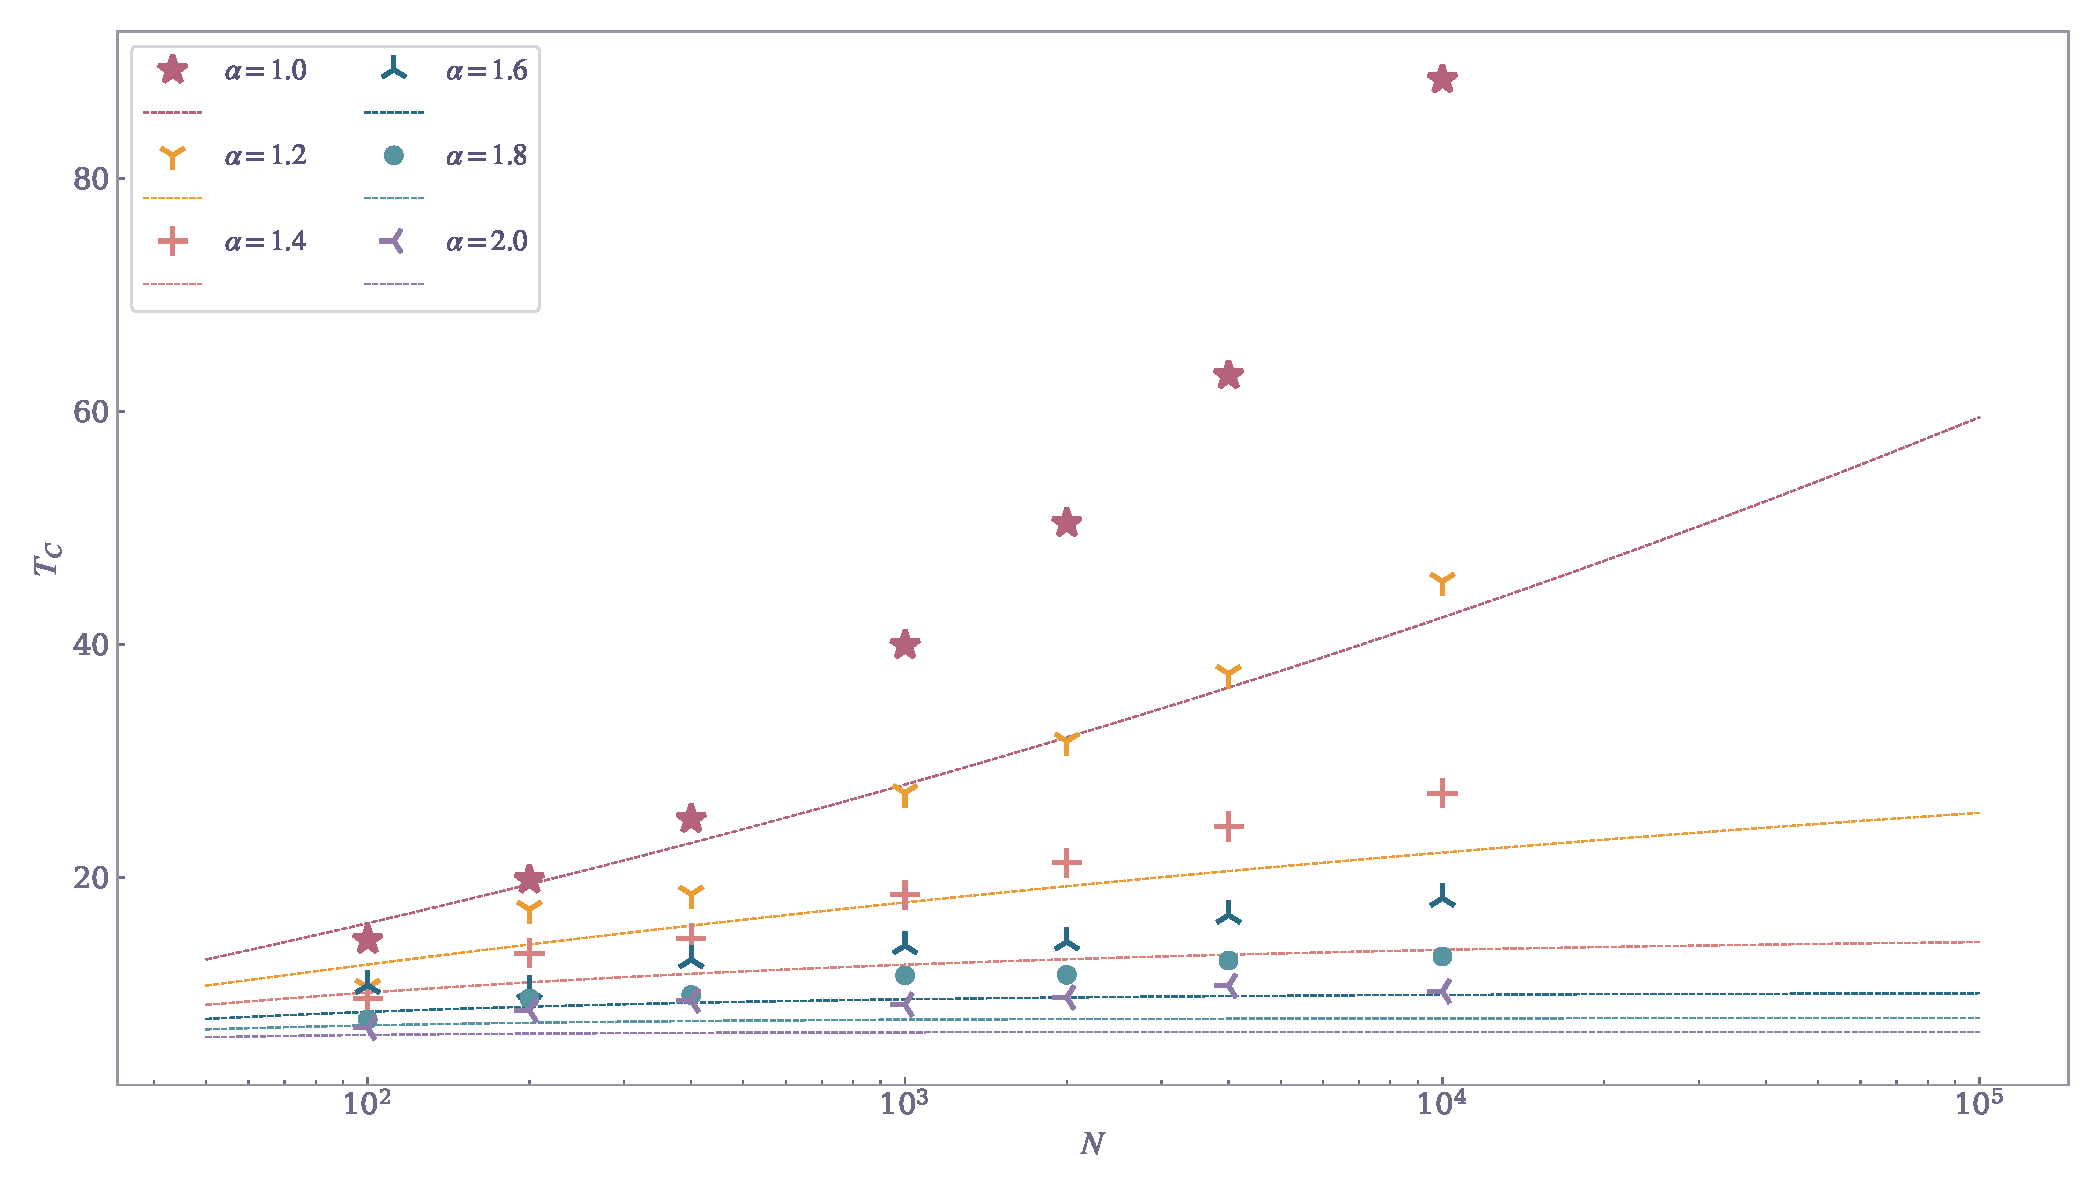
\includegraphics[width=\linewidth]{../figures/TC_vs_size.pdf}
\end{figure}

\todo{$e^{-\alpha k}$ vs. $1/k^\alpha$}


\end{document}
